\documentclass[1p]{elsarticle_modified}
%\bibliographystyle{elsarticle-num}

%\usepackage[colorlinks]{hyperref}
%\usepackage{abbrmath_seonhwa} %\Abb, \Ascr, \Acal ,\Abf, \Afrak
\usepackage{amsfonts}
\usepackage{amssymb}
\usepackage{amsmath}
\usepackage{amsthm}
\usepackage{scalefnt}
\usepackage{amsbsy}
\usepackage{kotex}
\usepackage{caption}
\usepackage{subfig}
\usepackage{color}
\usepackage{graphicx}
\usepackage{xcolor} %% white, black, red, green, blue, cyan, magenta, yellow
\usepackage{float}
\usepackage{setspace}
\usepackage{hyperref}

\usepackage{tikz}
\usetikzlibrary{arrows}

\usepackage{multirow}
\usepackage{array} % fixed length table
\usepackage{hhline}

%%%%%%%%%%%%%%%%%%%%%
\makeatletter
\renewcommand*\env@matrix[1][\arraystretch]{%
	\edef\arraystretch{#1}%
	\hskip -\arraycolsep
	\let\@ifnextchar\new@ifnextchar
	\array{*\c@MaxMatrixCols c}}
\makeatother %https://tex.stackexchange.com/questions/14071/how-can-i-increase-the-line-spacing-in-a-matrix
%%%%%%%%%%%%%%%

\usepackage[normalem]{ulem}

\newcommand{\msout}[1]{\ifmmode\text{\sout{\ensuremath{#1}}}\else\sout{#1}\fi}
%SOURCE: \msout is \stkout macro in https://tex.stackexchange.com/questions/20609/strikeout-in-math-mode

\newcommand{\cancel}[1]{
	\ifmmode
	{\color{red}\msout{#1}}
	\else
	{\color{red}\sout{#1}}
	\fi
}

\newcommand{\add}[1]{
	{\color{blue}\uwave{#1}}
}

\newcommand{\replace}[2]{
	\ifmmode
	{\color{red}\msout{#1}}{\color{blue}\uwave{#2}}
	\else
	{\color{red}\sout{#1}}{\color{blue}\uwave{#2}}
	\fi
}

\newcommand{\Sol}{\mathcal{S}} %segment
\newcommand{\D}{D} %diagram
\newcommand{\A}{\mathcal{A}} %arc


%%%%%%%%%%%%%%%%%%%%%%%%%%%%%5 test

\def\sl{\operatorname{\textup{SL}}(2,\Cbb)}
\def\psl{\operatorname{\textup{PSL}}(2,\Cbb)}
\def\quan{\mkern 1mu \triangleright \mkern 1mu}

\theoremstyle{definition}
\newtheorem{thm}{Theorem}[section]
\newtheorem{prop}[thm]{Proposition}
\newtheorem{lem}[thm]{Lemma}
\newtheorem{ques}[thm]{Question}
\newtheorem{cor}[thm]{Corollary}
\newtheorem{defn}[thm]{Definition}
\newtheorem{exam}[thm]{Example}
\newtheorem{rmk}[thm]{Remark}
\newtheorem{alg}[thm]{Algorithm}

\newcommand{\I}{\sqrt{-1}}
\begin{document}

%\begin{frontmatter}
%
%\title{Boundary parabolic representations of knots up to 8 crossings}
%
%%% Group authors per affiliation:
%\author{Yunhi Cho} 
%\address{Department of Mathematics, University of Seoul, Seoul, Korea}
%\ead{yhcho@uos.ac.kr}
%
%
%\author{Seonhwa Kim} %\fnref{s_kim}}
%\address{Center for Geometry and Physics, Institute for Basic Science, Pohang, 37673, Korea}
%\ead{ryeona17@ibs.re.kr}
%
%\author{Hyuk Kim}
%\address{Department of Mathematical Sciences, Seoul National University, Seoul 08826, Korea}
%\ead{hyukkim@snu.ac.kr}
%
%\author{Seokbeom Yoon}
%\address{Department of Mathematical Sciences, Seoul National University, Seoul, 08826,  Korea}
%\ead{sbyoon15@snu.ac.kr}
%
%\begin{abstract}
%We find all boundary parabolic representation of knots up to 8 crossings.
%
%\end{abstract}
%\begin{keyword}
%    \MSC[2010] 57M25 
%\end{keyword}
%
%\end{frontmatter}

%\linenumbers
%\tableofcontents
%
\newcommand\colored[1]{\textcolor{white}{\rule[-0.35ex]{0.8em}{1.4ex}}\kern-0.8em\color{red} #1}%
%\newcommand\colored[1]{\textcolor{white}{ #1}\kern-2.17ex	\textcolor{white}{ #1}\kern-1.81ex	\textcolor{white}{ #1}\kern-2.15ex\color{red}#1	}

{\Large $\underline{12a_{1158}~(K12a_{1158})}$}

\setlength{\tabcolsep}{10pt}
\renewcommand{\arraystretch}{1.6}
\vspace{1cm}\begin{tabular}{m{100pt}>{\centering\arraybackslash}m{274pt}}
\multirow{5}{120pt}{
	\centering
	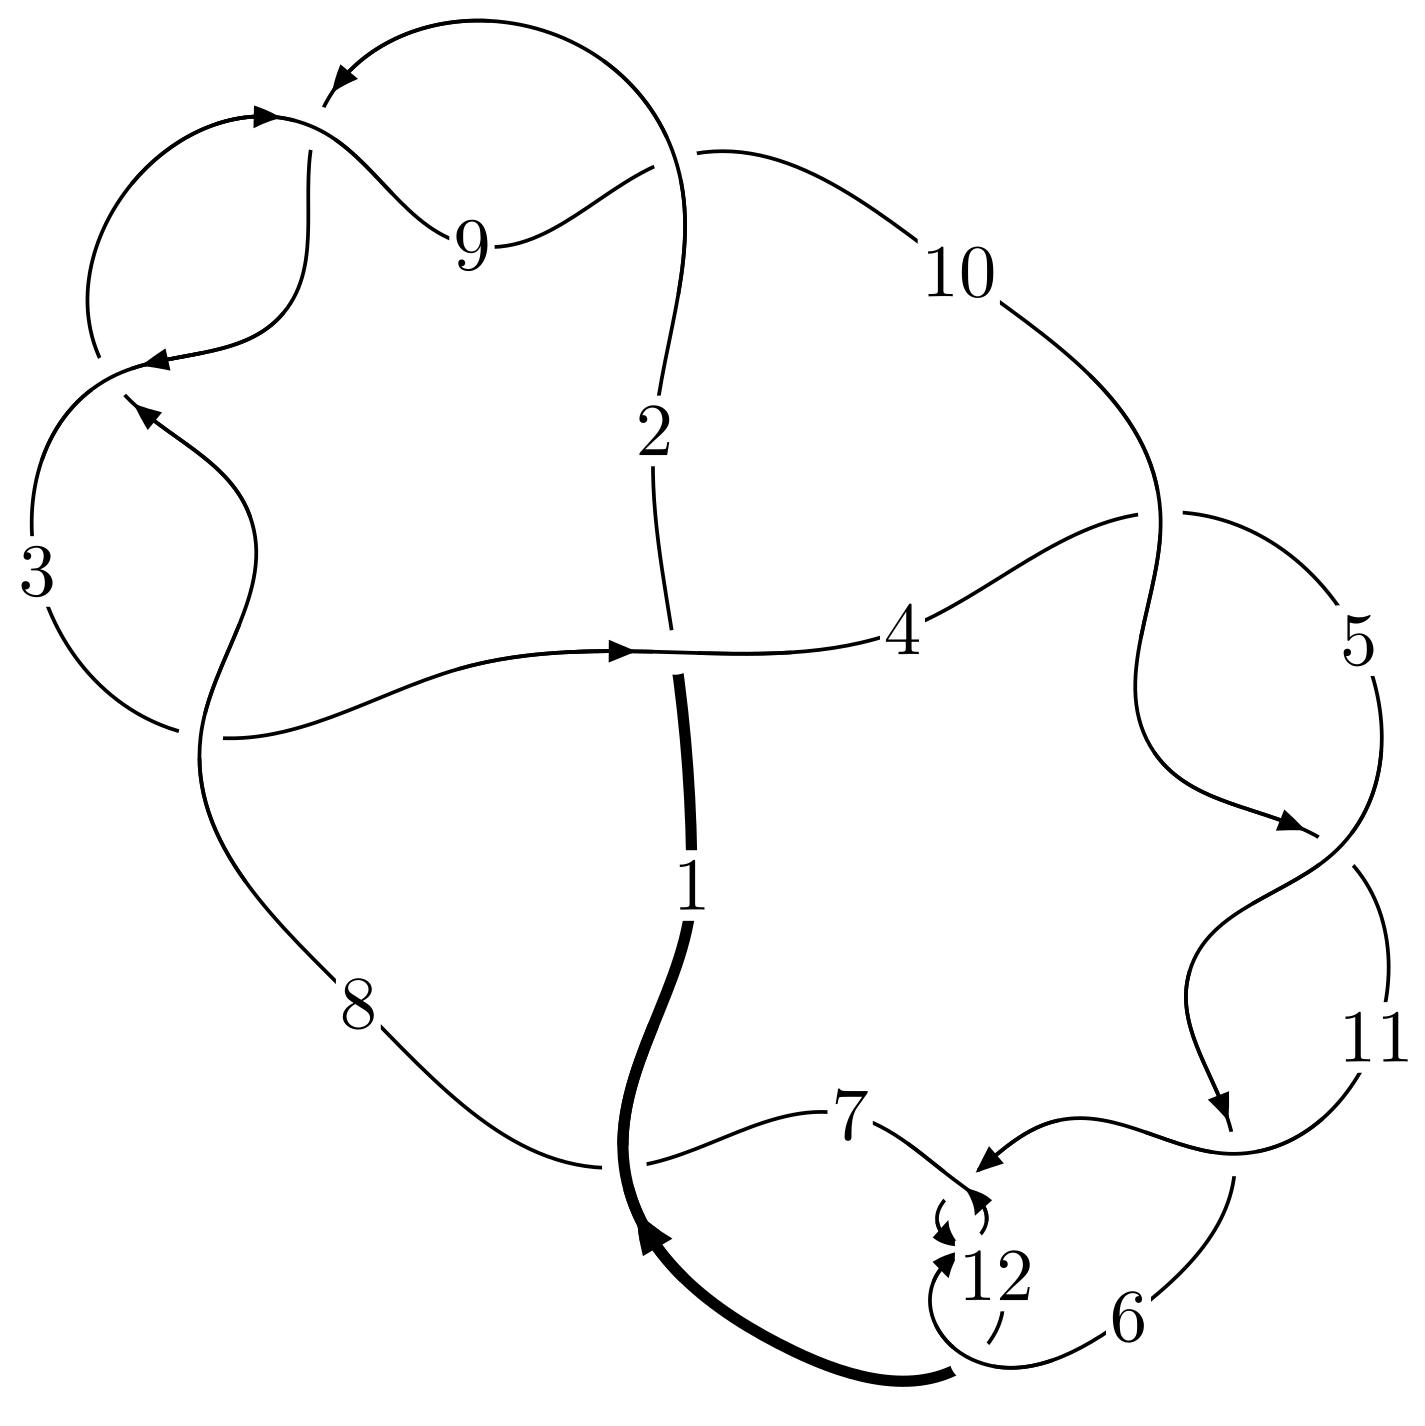
\includegraphics[width=112pt]{../../../GIT/diagram.site/Diagrams/png/1959_12a_1158.png}\\
\ \ \ A knot diagram\footnotemark}&
\allowdisplaybreaks
\textbf{Linearized knot diagam} \\
\cline{2-2}
 &
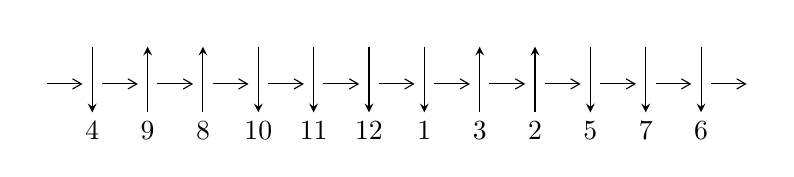
\begin{tikzpicture}[x=20pt, y=17pt]
	% nodes
	\node (C0) at (0, 0) {};
	\node (C1) at (1, 0) {};
	\node (C1U) at (1, +1) {};
	\node (C1D) at (1, -1) {4};

	\node (C2) at (2, 0) {};
	\node (C2U) at (2, +1) {};
	\node (C2D) at (2, -1) {9};

	\node (C3) at (3, 0) {};
	\node (C3U) at (3, +1) {};
	\node (C3D) at (3, -1) {8};

	\node (C4) at (4, 0) {};
	\node (C4U) at (4, +1) {};
	\node (C4D) at (4, -1) {10};

	\node (C5) at (5, 0) {};
	\node (C5U) at (5, +1) {};
	\node (C5D) at (5, -1) {11};

	\node (C6) at (6, 0) {};
	\node (C6U) at (6, +1) {};
	\node (C6D) at (6, -1) {12};

	\node (C7) at (7, 0) {};
	\node (C7U) at (7, +1) {};
	\node (C7D) at (7, -1) {1};

	\node (C8) at (8, 0) {};
	\node (C8U) at (8, +1) {};
	\node (C8D) at (8, -1) {3};

	\node (C9) at (9, 0) {};
	\node (C9U) at (9, +1) {};
	\node (C9D) at (9, -1) {2};

	\node (C10) at (10, 0) {};
	\node (C10U) at (10, +1) {};
	\node (C10D) at (10, -1) {5};

	\node (C11) at (11, 0) {};
	\node (C11U) at (11, +1) {};
	\node (C11D) at (11, -1) {7};

	\node (C12) at (12, 0) {};
	\node (C12U) at (12, +1) {};
	\node (C12D) at (12, -1) {6};
	\node (C13) at (13, 0) {};

	% arrows
	\draw[->,>={angle 60}]
	(C0) edge (C1) (C1) edge (C2) (C2) edge (C3) (C3) edge (C4) (C4) edge (C5) (C5) edge (C6) (C6) edge (C7) (C7) edge (C8) (C8) edge (C9) (C9) edge (C10) (C10) edge (C11) (C11) edge (C12) (C12) edge (C13) ;	\draw[->,>=stealth]
	(C1U) edge (C1D) (C2D) edge (C2U) (C3D) edge (C3U) (C4U) edge (C4D) (C5U) edge (C5D) (C6U) edge (C6D) (C7U) edge (C7D) (C8D) edge (C8U) (C9D) edge (C9U) (C10U) edge (C10D) (C11U) edge (C11D) (C12U) edge (C12D) ;
	\end{tikzpicture} \\
\hhline{~~} \\& 
\textbf{Solving Sequence} \\ \cline{2-2} 
 &
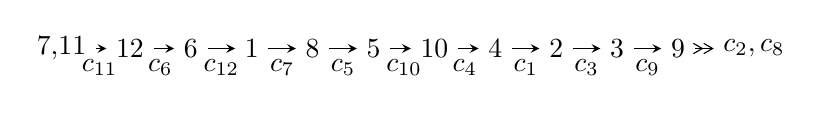
\begin{tikzpicture}[x=22pt, y=7pt]
	% node
	\node (A0) at (-1/8, 0) {7,11};
	\node (A1) at (1, 0) {12};
	\node (A2) at (2, 0) {6};
	\node (A3) at (3, 0) {1};
	\node (A4) at (4, 0) {8};
	\node (A5) at (5, 0) {5};
	\node (A6) at (6, 0) {10};
	\node (A7) at (7, 0) {4};
	\node (A8) at (8, 0) {2};
	\node (A9) at (9, 0) {3};
	\node (A10) at (10, 0) {9};
	\node (C1) at (1/2, -1) {$c_{11}$};
	\node (C2) at (3/2, -1) {$c_{6}$};
	\node (C3) at (5/2, -1) {$c_{12}$};
	\node (C4) at (7/2, -1) {$c_{7}$};
	\node (C5) at (9/2, -1) {$c_{5}$};
	\node (C6) at (11/2, -1) {$c_{10}$};
	\node (C7) at (13/2, -1) {$c_{4}$};
	\node (C8) at (15/2, -1) {$c_{1}$};
	\node (C9) at (17/2, -1) {$c_{3}$};
	\node (C10) at (19/2, -1) {$c_{9}$};
	\node (A11) at (45/4, 0) {$c_{2},c_{8}$};

	% edge
	\draw[->,>=stealth]	
	(A0) edge (A1) (A1) edge (A2) (A2) edge (A3) (A3) edge (A4) (A4) edge (A5) (A5) edge (A6) (A6) edge (A7) (A7) edge (A8) (A8) edge (A9) (A9) edge (A10) ;
	\draw[->>,>={angle 60}]	
	(A10) edge (A11);
\end{tikzpicture} \\ 

\end{tabular} \\

\footnotetext{
The image of knot diagram is generated by the software ``\textbf{Draw programme}" developed by Andrew Bartholomew(\url{http://www.layer8.co.uk/maths/draw/index.htm\#Running-draw}), where we modified some parts for our purpose(\url{https://github.com/CATsTAILs/LinksPainter}).
}\phantom \\ \newline 
\centering \textbf{Ideals for irreducible components\footnotemark of $X_{\text{par}}$} 
 
\begin{align*}
I^u_{1}&=\langle 
u^{38}- u^{37}+\cdots- u-1\rangle \\
\\
\end{align*}
\raggedright * 1 irreducible components of $\dim_{\mathbb{C}}=0$, with total 38 representations.\\
\footnotetext{All coefficients of polynomials are rational numbers. But the coefficients are sometimes approximated in decimal forms when there is not enough margin.}
\newpage
\renewcommand{\arraystretch}{1}
\centering \section*{I. $I^u_{1}= \langle u^{38}- u^{37}+\cdots- u-1 \rangle$}
\flushleft \textbf{(i) Arc colorings}\\
\begin{tabular}{m{7pt} m{180pt} m{7pt} m{180pt} }
\flushright $a_{7}=$&$\begin{pmatrix}0\\u\end{pmatrix}$ \\
\flushright $a_{11}=$&$\begin{pmatrix}1\\0\end{pmatrix}$ \\
\flushright $a_{12}=$&$\begin{pmatrix}1\\u^2\end{pmatrix}$ \\
\flushright $a_{6}=$&$\begin{pmatrix}u\\u^3+u\end{pmatrix}$ \\
\flushright $a_{1}=$&$\begin{pmatrix}u^2+1\\u^4+2 u^2\end{pmatrix}$ \\
\flushright $a_{8}=$&$\begin{pmatrix}- u^5-2 u^3- u\\- u^7-3 u^5-2 u^3+u\end{pmatrix}$ \\
\flushright $a_{5}=$&$\begin{pmatrix}u^3+2 u\\u^3+u\end{pmatrix}$ \\
\flushright $a_{10}=$&$\begin{pmatrix}- u^6-3 u^4-2 u^2+1\\- u^6-2 u^4- u^2\end{pmatrix}$ \\
\flushright $a_{4}=$&$\begin{pmatrix}- u^9-4 u^7-5 u^5+3 u\\- u^9-3 u^7-3 u^5+u\end{pmatrix}$ \\
\flushright $a_{2}=$&$\begin{pmatrix}- u^{22}-9 u^{20}+\cdots+4 u^2+1\\- u^{22}-8 u^{20}+\cdots-4 u^4+3 u^2\end{pmatrix}$ \\
\flushright $a_{3}=$&$\begin{pmatrix}- u^{21}-8 u^{19}+\cdots-4 u^3+3 u\\- u^{23}-9 u^{21}+\cdots+4 u^3+u\end{pmatrix}$ \\
\flushright $a_{9}=$&$\begin{pmatrix}- u^{37}-14 u^{35}+\cdots+10 u^3- u\\- u^{37}+u^{36}+\cdots- u-1\end{pmatrix}$\\&\end{tabular}
\flushleft \textbf{(ii) Obstruction class $= -1$}\\~\\
\flushleft \textbf{(iii) Cusp Shapes $= -4 u^{36}+4 u^{35}-56 u^{34}+52 u^{33}-352 u^{32}+304 u^{31}-1276 u^{30}+1024 u^{29}-2804 u^{28}+2080 u^{27}-3336 u^{26}+2240 u^{25}-364 u^{24}+36 u^{23}+5244 u^{22}-3388 u^{21}+7232 u^{20}-4040 u^{19}+1692 u^{18}-560 u^{17}-5000 u^{16}+2612 u^{15}-4528 u^{14}+1744 u^{13}+384 u^{12}-536 u^{11}+2024 u^{10}-736 u^9+416 u^8+104 u^7-368 u^6+192 u^5-84 u^4-12 u^3+24 u^2-12 u-6$}\\~\\
\newpage\renewcommand{\arraystretch}{1}
\flushleft \textbf{(iv) u-Polynomials at the component}\newline \\
\begin{tabular}{m{50pt}|m{274pt}}
Crossings & \hspace{64pt}u-Polynomials at each crossing \\
\hline $$\begin{aligned}c_{1}\end{aligned}$$&$\begin{aligned}
&u^{38}-13 u^{37}+\cdots-3409 u+723
\end{aligned}$\\
\hline $$\begin{aligned}c_{2},c_{3},c_{8}\\c_{9}\end{aligned}$$&$\begin{aligned}
&u^{38}+u^{37}+\cdots- u-1
\end{aligned}$\\
\hline $$\begin{aligned}c_{4},c_{5},c_{7}\\c_{10}\end{aligned}$$&$\begin{aligned}
&u^{38}+u^{37}+\cdots-9 u-5
\end{aligned}$\\
\hline $$\begin{aligned}c_{6},c_{11},c_{12}\end{aligned}$$&$\begin{aligned}
&u^{38}- u^{37}+\cdots- u-1
\end{aligned}$\\
\hline
\end{tabular}\\~\\
\newpage\renewcommand{\arraystretch}{1}
\flushleft \textbf{(v) Riley Polynomials at the component}\newline \\
\begin{tabular}{m{50pt}|m{274pt}}
Crossings & \hspace{64pt}Riley Polynomials at each crossing \\
\hline $$\begin{aligned}c_{1}\end{aligned}$$&$\begin{aligned}
&y^{38}-27 y^{37}+\cdots-8344645 y+522729
\end{aligned}$\\
\hline $$\begin{aligned}c_{2},c_{3},c_{8}\\c_{9}\end{aligned}$$&$\begin{aligned}
&y^{38}+45 y^{37}+\cdots+3 y+1
\end{aligned}$\\
\hline $$\begin{aligned}c_{4},c_{5},c_{7}\\c_{10}\end{aligned}$$&$\begin{aligned}
&y^{38}-47 y^{37}+\cdots-41 y+25
\end{aligned}$\\
\hline $$\begin{aligned}c_{6},c_{11},c_{12}\end{aligned}$$&$\begin{aligned}
&y^{38}+29 y^{37}+\cdots+3 y+1
\end{aligned}$\\
\hline
\end{tabular}\\~\\
\newpage\flushleft \textbf{(vi) Complex Volumes and Cusp Shapes}
$$\begin{array}{c|c|c}  
\text{Solutions to }I^u_{1}& \I (\text{vol} + \sqrt{-1}CS) & \text{Cusp shape}\\
 \hline 
\begin{aligned}
u &= \phantom{-}0.921549 + 0.026814 I\end{aligned}
 & \phantom{-}19.0082 - 5.9978 I & -13.8808 + 2.7631 I \\ \hline\begin{aligned}
u &= \phantom{-}0.921549 - 0.026814 I\end{aligned}
 & \phantom{-}19.0082 + 5.9978 I & -13.8808 - 2.7631 I \\ \hline\begin{aligned}
u &= -0.910401 + 0.016742 I\end{aligned}
 & -11.94600 + 3.74112 I & -12.20309 - 3.92212 I \\ \hline\begin{aligned}
u &= -0.910401 - 0.016742 I\end{aligned}
 & -11.94600 - 3.74112 I & -12.20309 + 3.92212 I \\ \hline\begin{aligned}
u &= \phantom{-}0.902816\phantom{ +0.000000I}\end{aligned}
 & -9.44212\phantom{ +0.000000I} & -8.29230\phantom{ +0.000000I} \\ \hline\begin{aligned}
u &= -0.295584 + 1.071570 I\end{aligned}
 & -8.32513 - 0.58329 I & -10.41542 - 0.50010 I \\ \hline\begin{aligned}
u &= -0.295584 - 1.071570 I\end{aligned}
 & -8.32513 + 0.58329 I & -10.41542 + 0.50010 I \\ \hline\begin{aligned}
u &= \phantom{-}0.220657 + 1.122970 I\end{aligned}
 & -0.206300 - 0.496209 I & -9.24627 - 0.65693 I \\ \hline\begin{aligned}
u &= \phantom{-}0.220657 - 1.122970 I\end{aligned}
 & -0.206300 + 0.496209 I & -9.24627 + 0.65693 I \\ \hline\begin{aligned}
u &= -0.203175 + 1.232690 I\end{aligned}
 & \phantom{-}2.53092 + 2.66616 I & -0.99392 - 3.01578 I \\ \hline\begin{aligned}
u &= -0.203175 - 1.232690 I\end{aligned}
 & \phantom{-}2.53092 - 2.66616 I & -0.99392 + 3.01578 I \\ \hline\begin{aligned}
u &= -0.033249 + 1.263780 I\end{aligned}
 & \phantom{-}4.26230 + 1.45522 I & \phantom{-}1.17782 - 5.08792 I \\ \hline\begin{aligned}
u &= -0.033249 - 1.263780 I\end{aligned}
 & \phantom{-}4.26230 - 1.45522 I & \phantom{-}1.17782 + 5.08792 I \\ \hline\begin{aligned}
u &= \phantom{-}0.247059 + 1.268440 I\end{aligned}
 & \phantom{-}1.06826 - 5.79649 I & -5.38275 + 8.72620 I \\ \hline\begin{aligned}
u &= \phantom{-}0.247059 - 1.268440 I\end{aligned}
 & \phantom{-}1.06826 + 5.79649 I & -5.38275 - 8.72620 I \\ \hline\begin{aligned}
u &= -0.689534 + 0.138578 I\end{aligned}
 & -11.05530 + 4.25242 I & -13.45193 - 4.29885 I \\ \hline\begin{aligned}
u &= -0.689534 - 0.138578 I\end{aligned}
 & -11.05530 - 4.25242 I & -13.45193 + 4.29885 I \\ \hline\begin{aligned}
u &= \phantom{-}0.087911 + 1.303620 I\end{aligned}
 & -2.26439 - 2.76931 I & -3.18945 + 3.50256 I \\ \hline\begin{aligned}
u &= \phantom{-}0.087911 - 1.303620 I\end{aligned}
 & -2.26439 + 2.76931 I & -3.18945 - 3.50256 I \\ \hline\begin{aligned}
u &= -0.275003 + 1.294930 I\end{aligned}
 & -6.60950 + 7.69625 I & -7.73538 - 6.48615 I \\ \hline\begin{aligned}
u &= -0.275003 - 1.294930 I\end{aligned}
 & -6.60950 - 7.69625 I & -7.73538 + 6.48615 I \\ \hline\begin{aligned}
u &= \phantom{-}0.456153 + 1.266600 I\end{aligned}
 & -16.6317 + 1.0857 I & -10.74929 + 0. I\phantom{ +0.000000I} \\ \hline\begin{aligned}
u &= \phantom{-}0.456153 - 1.266600 I\end{aligned}
 & -16.6317 - 1.0857 I & -10.74929 + 0. I\phantom{ +0.000000I} \\ \hline\begin{aligned}
u &= -0.443090 + 1.271380 I\end{aligned}
 & -8.05649 + 1.09065 I & -9.00721 + 0. I\phantom{ +0.000000I} \\ \hline\begin{aligned}
u &= -0.443090 - 1.271380 I\end{aligned}
 & -8.05649 - 1.09065 I & -9.00721 + 0. I\phantom{ +0.000000I} \\ \hline\begin{aligned}
u &= \phantom{-}0.432187 + 1.283350 I\end{aligned}
 & -5.45541 - 4.77115 I & -4.00000 + 2.96319 I \\ \hline\begin{aligned}
u &= \phantom{-}0.432187 - 1.283350 I\end{aligned}
 & -5.45541 + 4.77115 I & -4.00000 - 2.96319 I \\ \hline\begin{aligned}
u &= \phantom{-}0.626097 + 0.102774 I\end{aligned}
 & -3.13828 - 2.66124 I & -12.32538 + 6.29351 I \\ \hline\begin{aligned}
u &= \phantom{-}0.626097 - 0.102774 I\end{aligned}
 & -3.13828 + 2.66124 I & -12.32538 - 6.29351 I \\ \hline\begin{aligned}
u &= -0.433822 + 1.297770 I\end{aligned}
 & -7.85499 + 8.54454 I & -8.56346 - 6.86027 I\\
 \hline 
 \end{array}$$\newpage$$\begin{array}{c|c|c}  
\text{Solutions to }I^u_{1}& \I (\text{vol} + \sqrt{-1}CS) & \text{Cusp shape}\\
 \hline 
\begin{aligned}
u &= -0.433822 - 1.297770 I\end{aligned}
 & -7.85499 - 8.54454 I & -8.56346 + 6.86027 I \\ \hline\begin{aligned}
u &= \phantom{-}0.438829 + 1.307920 I\end{aligned}
 & -16.3117 - 10.8564 I & -10.31831 + 5.56337 I \\ \hline\begin{aligned}
u &= \phantom{-}0.438829 - 1.307920 I\end{aligned}
 & -16.3117 + 10.8564 I & -10.31831 - 5.56337 I \\ \hline\begin{aligned}
u &= \phantom{-}0.354367 + 0.402887 I\end{aligned}
 & -7.36308 - 1.41419 I & -9.22771 + 4.33033 I \\ \hline\begin{aligned}
u &= \phantom{-}0.354367 - 0.402887 I\end{aligned}
 & -7.36308 + 1.41419 I & -9.22771 - 4.33033 I \\ \hline\begin{aligned}
u &= -0.535584\phantom{ +0.000000I}\end{aligned}
 & -1.19956\phantom{ +0.000000I} & -7.62450\phantom{ +0.000000I} \\ \hline\begin{aligned}
u &= -0.184566 + 0.290087 I\end{aligned}
 & -0.222289 + 0.830054 I & -5.72806 - 8.07347 I \\ \hline\begin{aligned}
u &= -0.184566 - 0.290087 I\end{aligned}
 & -0.222289 - 0.830054 I & -5.72806 + 8.07347 I\\
 \hline 
 \end{array}$$\newpage
\newpage\renewcommand{\arraystretch}{1}
\centering \section*{ II. u-Polynomials}
\begin{tabular}{m{50pt}|m{274pt}}
Crossings & \hspace{64pt}u-Polynomials at each crossing \\
\hline $$\begin{aligned}c_{1}\end{aligned}$$&$\begin{aligned}
&u^{38}-13 u^{37}+\cdots-3409 u+723
\end{aligned}$\\
\hline $$\begin{aligned}c_{2},c_{3},c_{8}\\c_{9}\end{aligned}$$&$\begin{aligned}
&u^{38}+u^{37}+\cdots- u-1
\end{aligned}$\\
\hline $$\begin{aligned}c_{4},c_{5},c_{7}\\c_{10}\end{aligned}$$&$\begin{aligned}
&u^{38}+u^{37}+\cdots-9 u-5
\end{aligned}$\\
\hline $$\begin{aligned}c_{6},c_{11},c_{12}\end{aligned}$$&$\begin{aligned}
&u^{38}- u^{37}+\cdots- u-1
\end{aligned}$\\
\hline
\end{tabular}\newpage\renewcommand{\arraystretch}{1}
\centering \section*{ III. Riley Polynomials}
\begin{tabular}{m{50pt}|m{274pt}}
Crossings & \hspace{64pt}Riley Polynomials at each crossing \\
\hline $$\begin{aligned}c_{1}\end{aligned}$$&$\begin{aligned}
&y^{38}-27 y^{37}+\cdots-8344645 y+522729
\end{aligned}$\\
\hline $$\begin{aligned}c_{2},c_{3},c_{8}\\c_{9}\end{aligned}$$&$\begin{aligned}
&y^{38}+45 y^{37}+\cdots+3 y+1
\end{aligned}$\\
\hline $$\begin{aligned}c_{4},c_{5},c_{7}\\c_{10}\end{aligned}$$&$\begin{aligned}
&y^{38}-47 y^{37}+\cdots-41 y+25
\end{aligned}$\\
\hline $$\begin{aligned}c_{6},c_{11},c_{12}\end{aligned}$$&$\begin{aligned}
&y^{38}+29 y^{37}+\cdots+3 y+1
\end{aligned}$\\
\hline
\end{tabular}
\vskip 2pc
\end{document}